\documentclass{standalone}
\usepackage{tikz}
\usetikzlibrary{arrows.meta, positioning}

\begin{document}
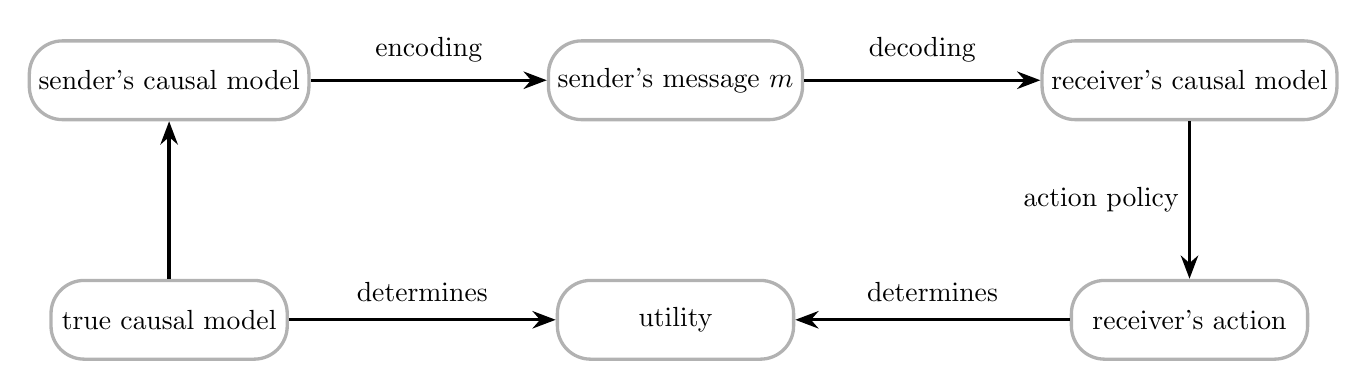
\begin{tikzpicture}[>=Stealth, line width=1.2pt,
  every node/.style={draw=gray!60, rounded corners=12pt, minimum width=3cm, minimum height = 1cm}]

  % Nodes
  \node (S) []  {sender's causal model};
  \node (M) [right=3cm of S] {sender's message $m$};
  \node (R) [right=3cm of M] {receiver's causal model};
  \node (W) [below=2cm of S] {true causal model};
  \node (U) [below=2cm of M] {utility};
  \node (A) [below=2cm of R] {receiver's action};

  % Edges
  \draw[->] (W)  -- node[midway, right, draw=none, minimum size=0pt] {} (S);
  \draw[->] (S)  -- node[midway, above=0.1cm, draw=none, minimum size=0pt] {encoding} (M);
  \draw[->] (M)  -- node[midway, above=0.1cm, draw=none, minimum size=0pt] {decoding} (R);
  \draw[->] (R)  -- node[midway, left, draw=none, minimum size=0pt] {action policy} (A);
  \draw[->] (A)  -- node[midway, above=0.1cm, draw=none, minimum size=0pt] {determines} (U);
  \draw[->] (W)  -- node[midway, above=0.1cm, draw=none, minimum size=0pt] {determines} (U);

\end{tikzpicture}
\end{document}
